\section[Interfaz OSC]{Más allá de la pantalla: interfaz OSC}
%\sectionmark{Interfaz OSC}
\label{sec:osc}

\textit{Open Sound Control}, conocido por sus siglas OSC, es, tal como lo define la propia CNMAT (\textit{Center for New Music and Audio Technologies}), <<un protocolo para la comunicación entre computadoras, sintetizadores y otros dispositivos multimedia, optimizado para la tecnología en red>>. Nacido en el CNMAT, OSC busca ser un MIDI mejorado, especialmente en lo que se refiere a la facilidad de implementación, precisión de los datos y a la expresividad de su sintaxis. Un mensaje OSC está formado por una cadena de texto en estilo URL, y los valores formados por 32 bits, tanto enteros como de coma flotante. 

Por todo esto, y por su fácil uso en SuperCollider, este protocolo ha sido escogido, no solo para que la clase \className\  se comunique con interfaces remotas, sino cualquier comunicación con ella se produce a través de este protocolo. Se ha creado un único método en la clase con el que el usuario puede interactuar de forma segura: \texttt{\className.setParameterOSC (string, value, addrForbidden)}. \texttt{string} es la cadena de texto del mensaje y \texttt{value}, el valor. Ambos forman el mensaje OSC que se envía al sintetizador. Tanto si los valores se introducen desde la red, como desde la interfaz gráfica por defecto como a través de mensajes de texto de código, el método recomendado es precisamente este.

Todo mensaje recibido por el sintetizador es devuelto, a modo de eco, a todas las direcciones con las que el sintetizador ha sido <<emparejado>> previamente. El emparejamiento de los diversos dispositivos al sintetizador se realiza por medio del método \texttt{\className.pairDevice()}, reconociendo cualquier dispositivo en red que envíe el mensaje \texttt{/ping} en los siguientes 4 segundos\footnote{Este mensaje se ha elegido para mantener compatibilidad con el software \textit{TouchOSC} (\texttt{https://hexler.net/products/touchosc}, una App para dispositivos móviles que permite diseñar interfaces eficientes y muy funcionales, usando el protocolo OSC)}. El argumento \texttt{addrFrobidden} del método de envío de mensajes OSC contendrá opcionalmente la dirección del dispositivo remitente, y está pensado para bloquear dicha dirección a la hora de hacer eco del mensaje.

\appName trae un ejemplo de interfaz OSC implementada en \textit{TouchOSC} (fig. \ref{fig:touchOSC}), en la carpeta \texttt{[raíz]/TouchOSC}. Contiene algunos ejemplos de módulos así como las dos matrices de conexiones (sección \ref{sec:patchbay}).

\begin{figure}
	\centering
	\begin{subfigure}[b]{0.3\textwidth}
		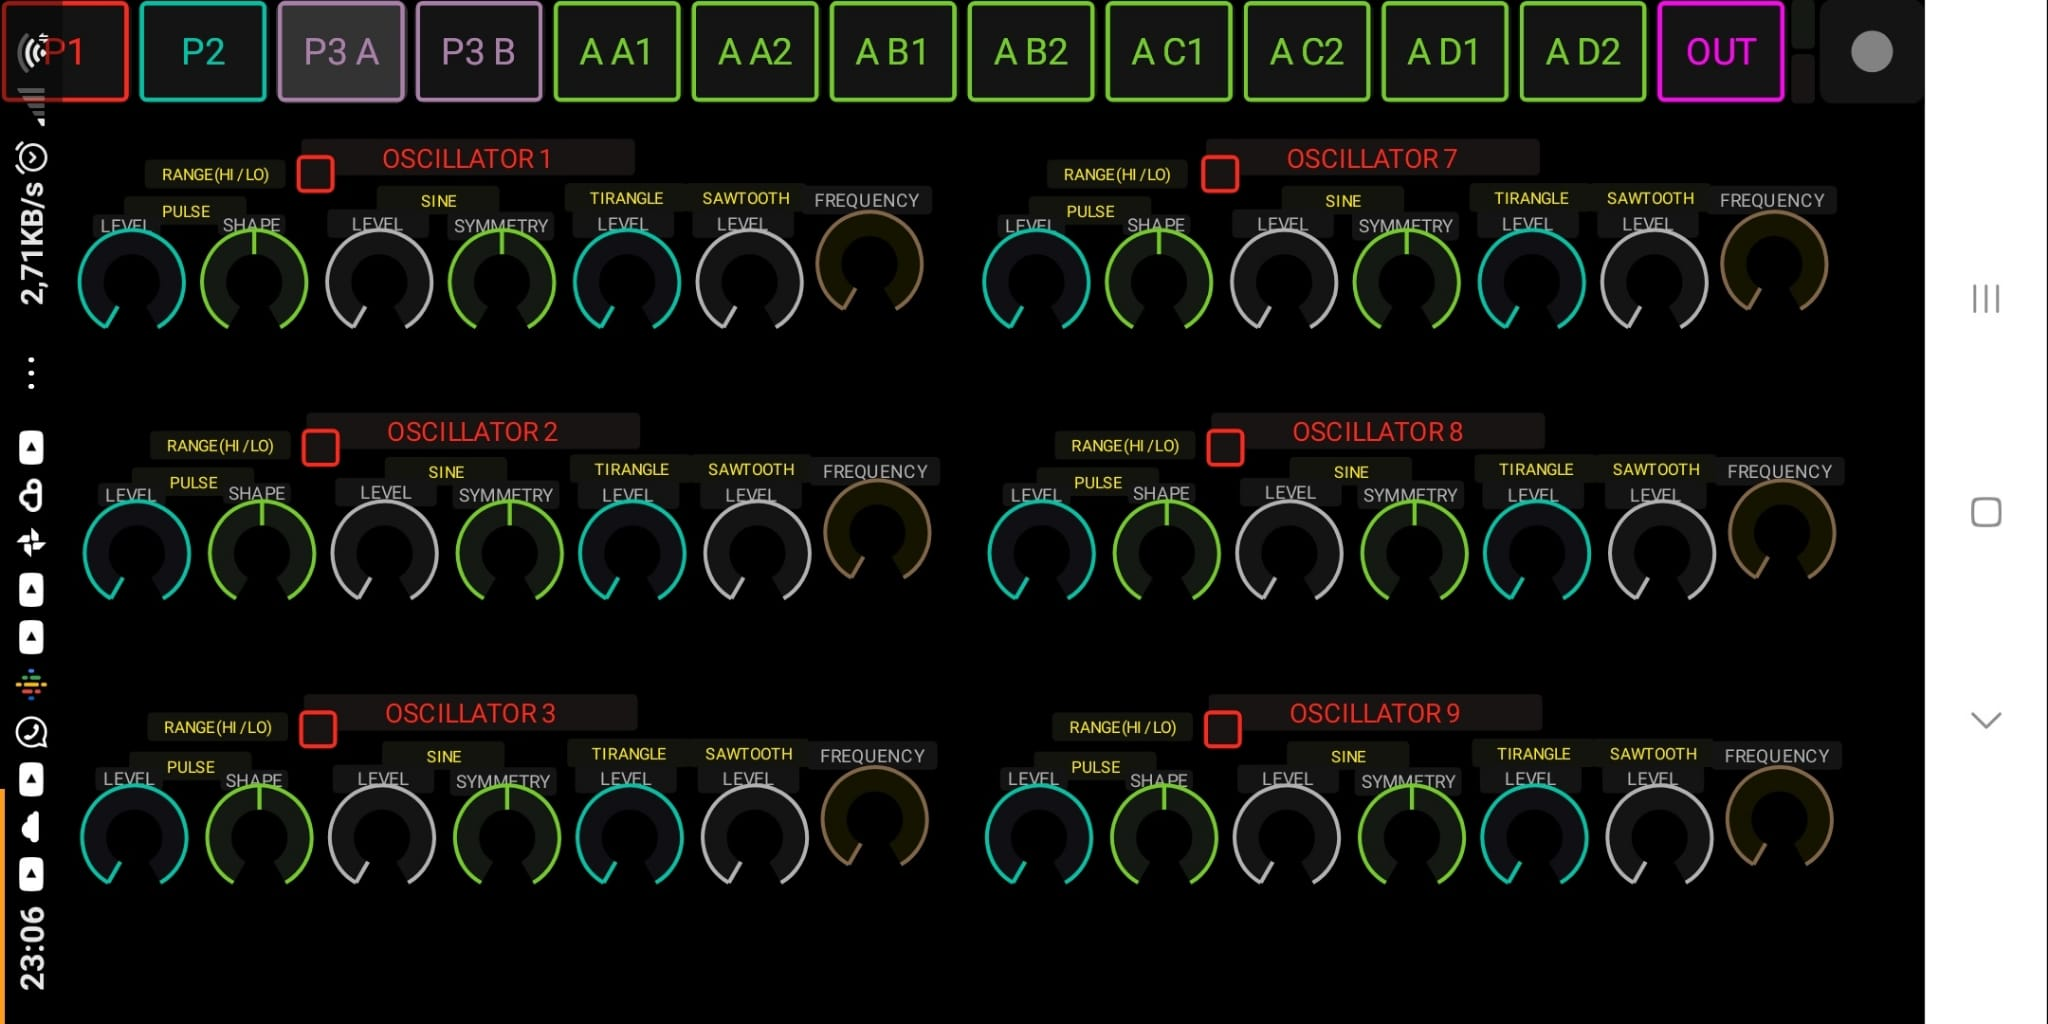
\includegraphics[width=\textwidth]{images/touchOSC_oscillators}
		\caption{Algunos osciladores}
		\label{fig:touchOSC_oscillators}
	\end{subfigure}
	~ %add desired spacing between images, e. g. ~, \quad, \qquad, \hfill etc. 
	%(or a blank line to force the subfigure onto a new line)
	\begin{subfigure}[b]{0.3\textwidth}
		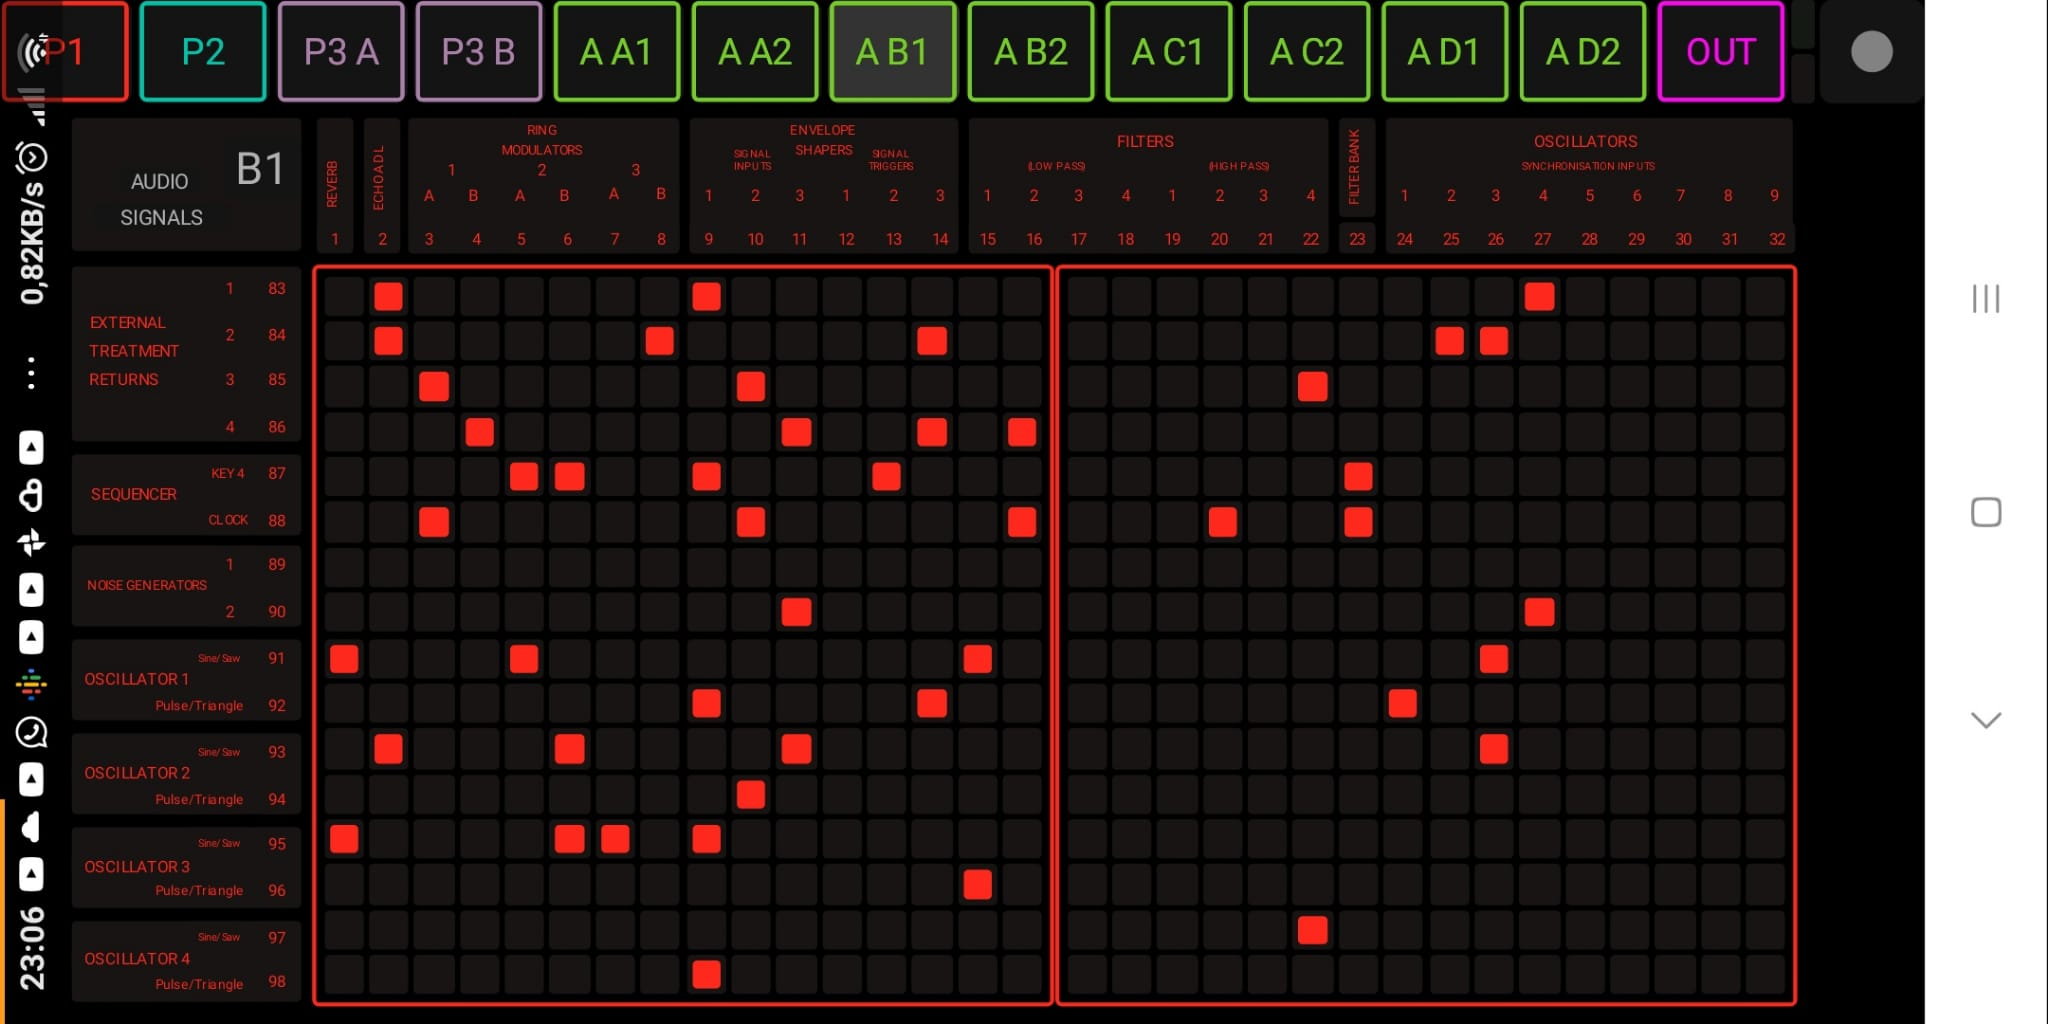
\includegraphics[width=\textwidth]{images/touchOSC_matriz}
		\caption{Matriz de audio}
		\label{fig:touchOSC_matriz}
	\end{subfigure}
	~ %add desired spacing between images, e. g. ~, \quad, \qquad, \hfill etc. 
	%(or a blank line to force the subfigure onto a new line)
	\begin{subfigure}[b]{0.3\textwidth}
		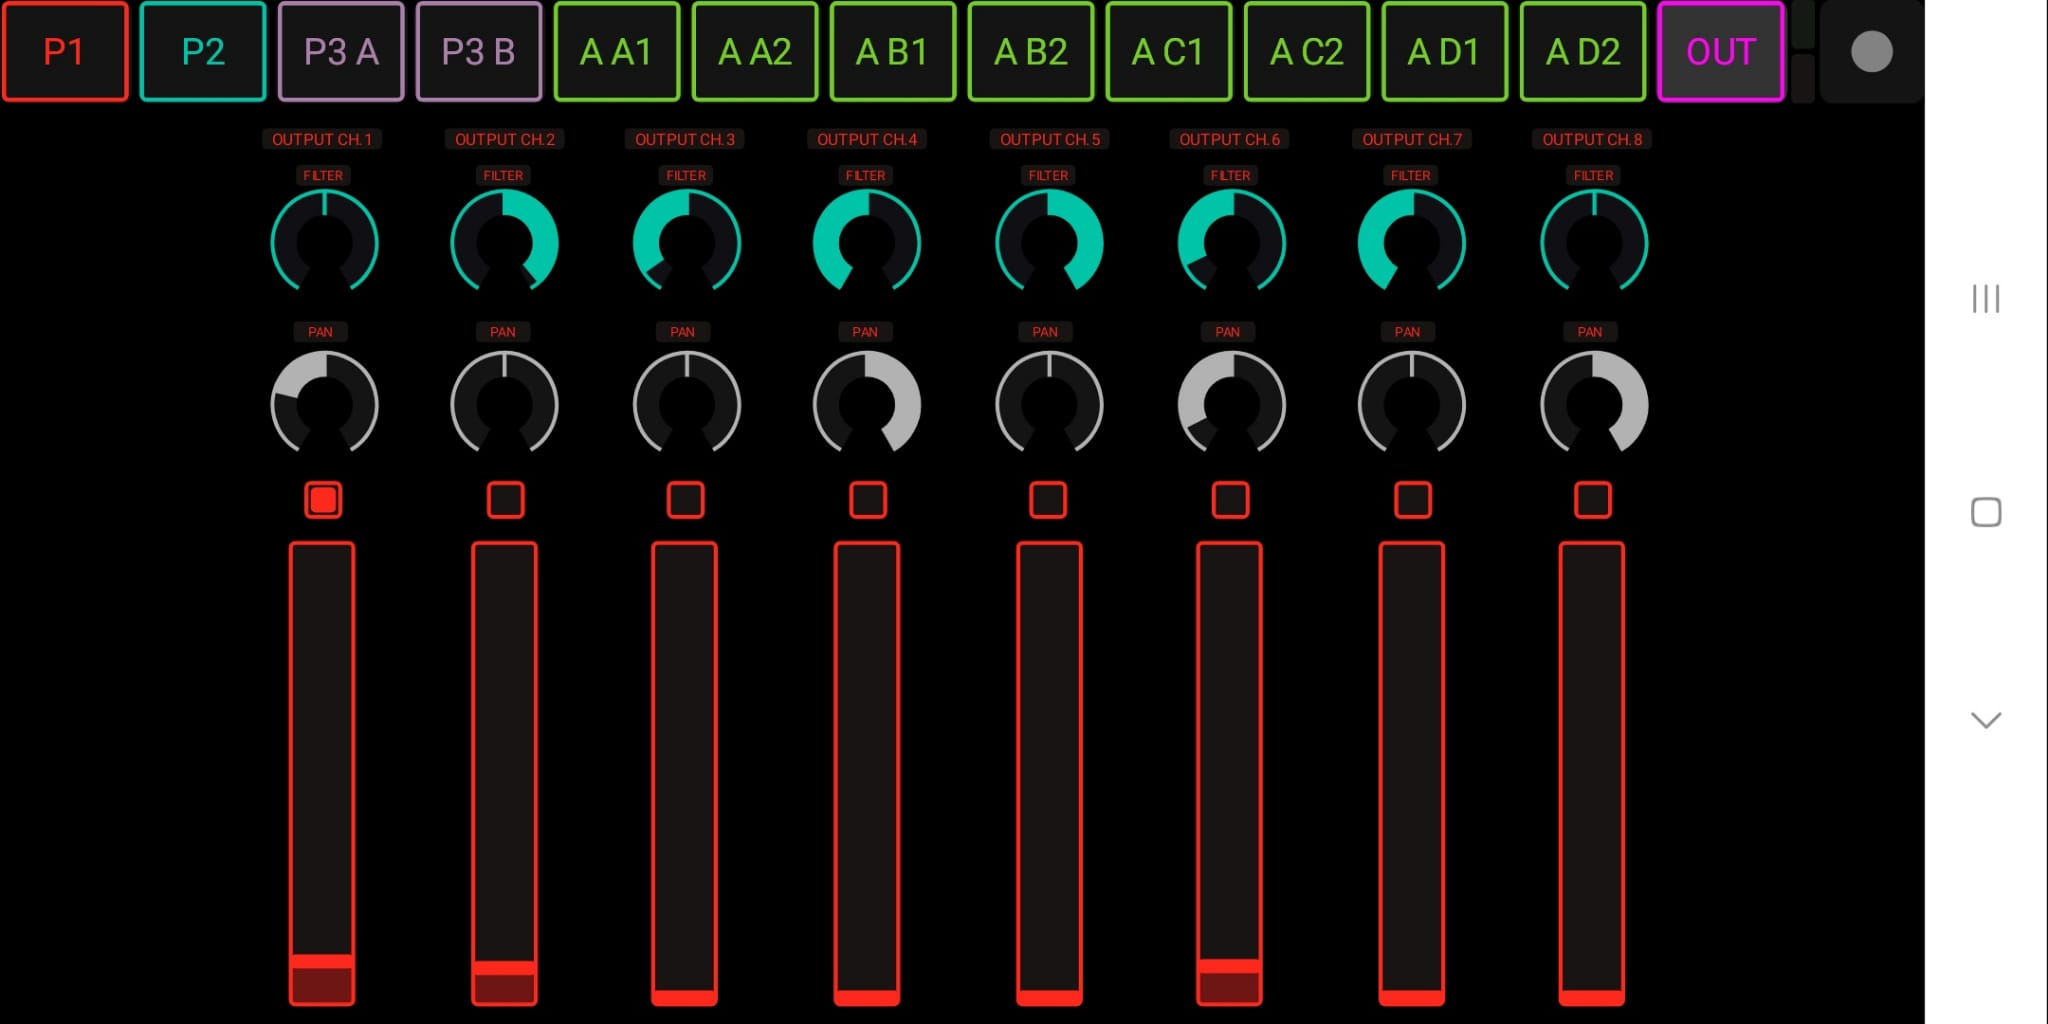
\includegraphics[width=\textwidth]{images/touchOSC_channels}
		\caption{\textit{Output channels}}
		\label{fig:touchOSC_channels}
	\end{subfigure}
	\caption{Páginas de ejemplo del \textit{layout} creado en \textit{TouchOSC}. Los \textit{widgets} se pueden deslizar y girar con el dedo en pantallas táctiles.}
	\label{fig:touchOSC}
\end{figure}

Esta interfaz única de comunicación de la clase \className\ con el exterior extiende las posibilidades de uso de este dispositivo más allá de la propia interfaz gráfica por defecto. Podemos imaginar interfaces en red creadas ad hoc, escritas en cualquier lenguaje de programación y framework o, quizás algo mucho más sugerente y creativo, interfaces de hardware controladas con microchips tipo Arduino. Por esta razón se ha cuidado que los mensajes OSC necesarios para comunicarse con el sintetizador sean autoexplicativos. En la tabla \ref{table:osc} se recoge la formación de todos los mensajes OSC que entiende la clase \texttt{\className}, asociados a cada uno de los módulos.

\begin{table}
	\begin{center}
		\begin{tabular}{ l c l l l }
			\multicolumn{3}{c}{\textit{OSC Type Tag String}} \\
			\cline{1-3}
			Módulo			& Número			& Parámetro				& \textit{Level} 	& Módulo de Synthi 100 \\
			
			% Módulo de Envelope Shaper.
			\hline 
			\multirow{9}{*}{\texttt{/env}}	& \multirow{9}{*}{\texttt{/$[1-3]$}}
			& \texttt{/selector}	&\texttt{[1-5]} & \multirow{9}{*}{\textit{Envelope Shapers}}\\
			& & \texttt{/delay} & $[0.0-10.0]$ & \\
			& & \texttt{/attack} & \texttt{[0.0-10.0]} & \\
			& & \texttt{/decay} & \texttt{[0.0-10.0]} &\\
			& & \texttt{/sustain} & \texttt{[0.0-10.0]}  &\\
			& & \texttt{/release} & \texttt{[0.0-10.0]} &\\
			& & \texttt{/envelopeLevel} & \texttt{[-5.0-5.0]} &\\
			& & \texttt{/signalLevel} & \texttt{[-5.0-5.0]} &\\
			& & \texttt{/gate} & \texttt{[0-1]} &\\
			\hline
			
			% Módulo de Ring Modulator.
			\multirow{1}{*}{\texttt{/ring}}	& \multirow{1}{*}{\texttt{/[1-2]}}	& \texttt{/level}	&\texttt{[0.0-10.0]} & \multirow{1}{*}{\textit{Ring Modulators}}\\
			\hline
			
			% Módulo de oscilador.
			\hline 
			\multirow{8}{*}{\texttt{/osc}}	& \multirow{8}{*}{\texttt{/[1-12]}}	& \texttt{/pulse/level}	&\texttt{[0.0-10.0]} & \multirow{8}{*}{\textit{Oscillators}}\\
			& & \texttt{/pulse/shape} & \texttt{[-5.0-5.0]} & \\
			& & \texttt{/sine/level} & \texttt{[0.0-10.0]} & \\
			& & \texttt{/sine/symmetry} & \texttt{[-5.0-5.0]} &\\
			& & \texttt{/triangle/level} & \texttt{[0.0-10.0]}  &\\
			& & \texttt{/sawtooth/level} & \texttt{[0.0-10.0]} &\\
			& & \texttt{/frequency} & \texttt{[0.0-10.0]} &\\
			& & \texttt{/range} & \texttt{[0-1]} &\\
			
			% Módulo de Noise generator
			\hline
			\multirow{2}{*}{\texttt{/noise}}	& \multirow{2}{*}{\texttt{/[1-2]}}	& \texttt{/color}	&\texttt{[0.0-10.0]} & \multirow{2}{*}{\textit{Noise Generators}}\\
			& & \texttt{/level} &\texttt{[0.0-10.0]}& \\
			\hline
			
			% Módulo de Random control voltage generator
			\hline
			\multirow{5}{*}{\texttt{/random}}	& 	& \texttt{/mean}	&\texttt{[0.0-10.0]} \\
			& & \texttt{/variance} &\texttt{[-5.0-5.0]}&  \multirow{2}{*}{\textit{Random Control}}\\
			& & \texttt{/voltage1} &\texttt{[0.0-10.0]}& \multirow{2}{*}{\textit{Voltage Generator}}\\
			& & \texttt{/voltage2} &\texttt{[0.0-10.0]}& \\
			& & \texttt{/key} &\texttt{[-5.0-5.0]}& \\
			\hline
			
			% Módulo de Output channels
			\multirow{4}{*}{\texttt{/out}}	& \multirow{4}{*}{\texttt{/[1-8]}}	& \texttt{/filter}	&\texttt{[-5.0-5.0]} & \multirow{4}{*}{\textit{Input Amplifiers}}\\
			& & \texttt{/pan} & \texttt{[-5.0-5.0]} & \\
			& & \texttt{/on} & \texttt{[0-1]} & \\
			& & \texttt{/level} & \texttt{[0.0-10.0]} &\\
			\hline
			
			% Módulo de Input Amplifiers
			\multirow{1}{*}{\texttt{/in}}	& \multirow{1}{*}{\texttt{/[1-8]}}	& \texttt{/level}	&\texttt{[0.0-10.0]} & \multirow{1}{*}{\textit{Output Channels}}\\
			\hline
			
			% Módulo de Patchbay de Audio
			\multirow{1}{*}{\texttt{/patchA}}	& 	
			& \texttt{/[67-128]/[1-66]} 	&\texttt{[0.0-1.0]} & \multirow{1}{*}{\textit{Audio Control}}\\
			\hline
			
			% Módulo de Patchbay de Voltaje
			\multirow{1}{*}{\texttt{/patchV}}	& 	
			& \texttt{/[67-128]/[1-66]} 	&\texttt{[0.0-1.0]} & \multirow{1}{*}{\textit{Voltage Control}}\\
			\hline
			
		\end{tabular}
		\caption[Estructura de los mensajes OSC]{Estructura de la cadena de texto (\textit{OSC Type Tag String}) y valor de los mensajes OSC para comunicarse con \className.}
		\label{table:osc}
	\end{center}
\end{table}